\section{L. Cylinder Results}

\begin{figure}[t]
\centering
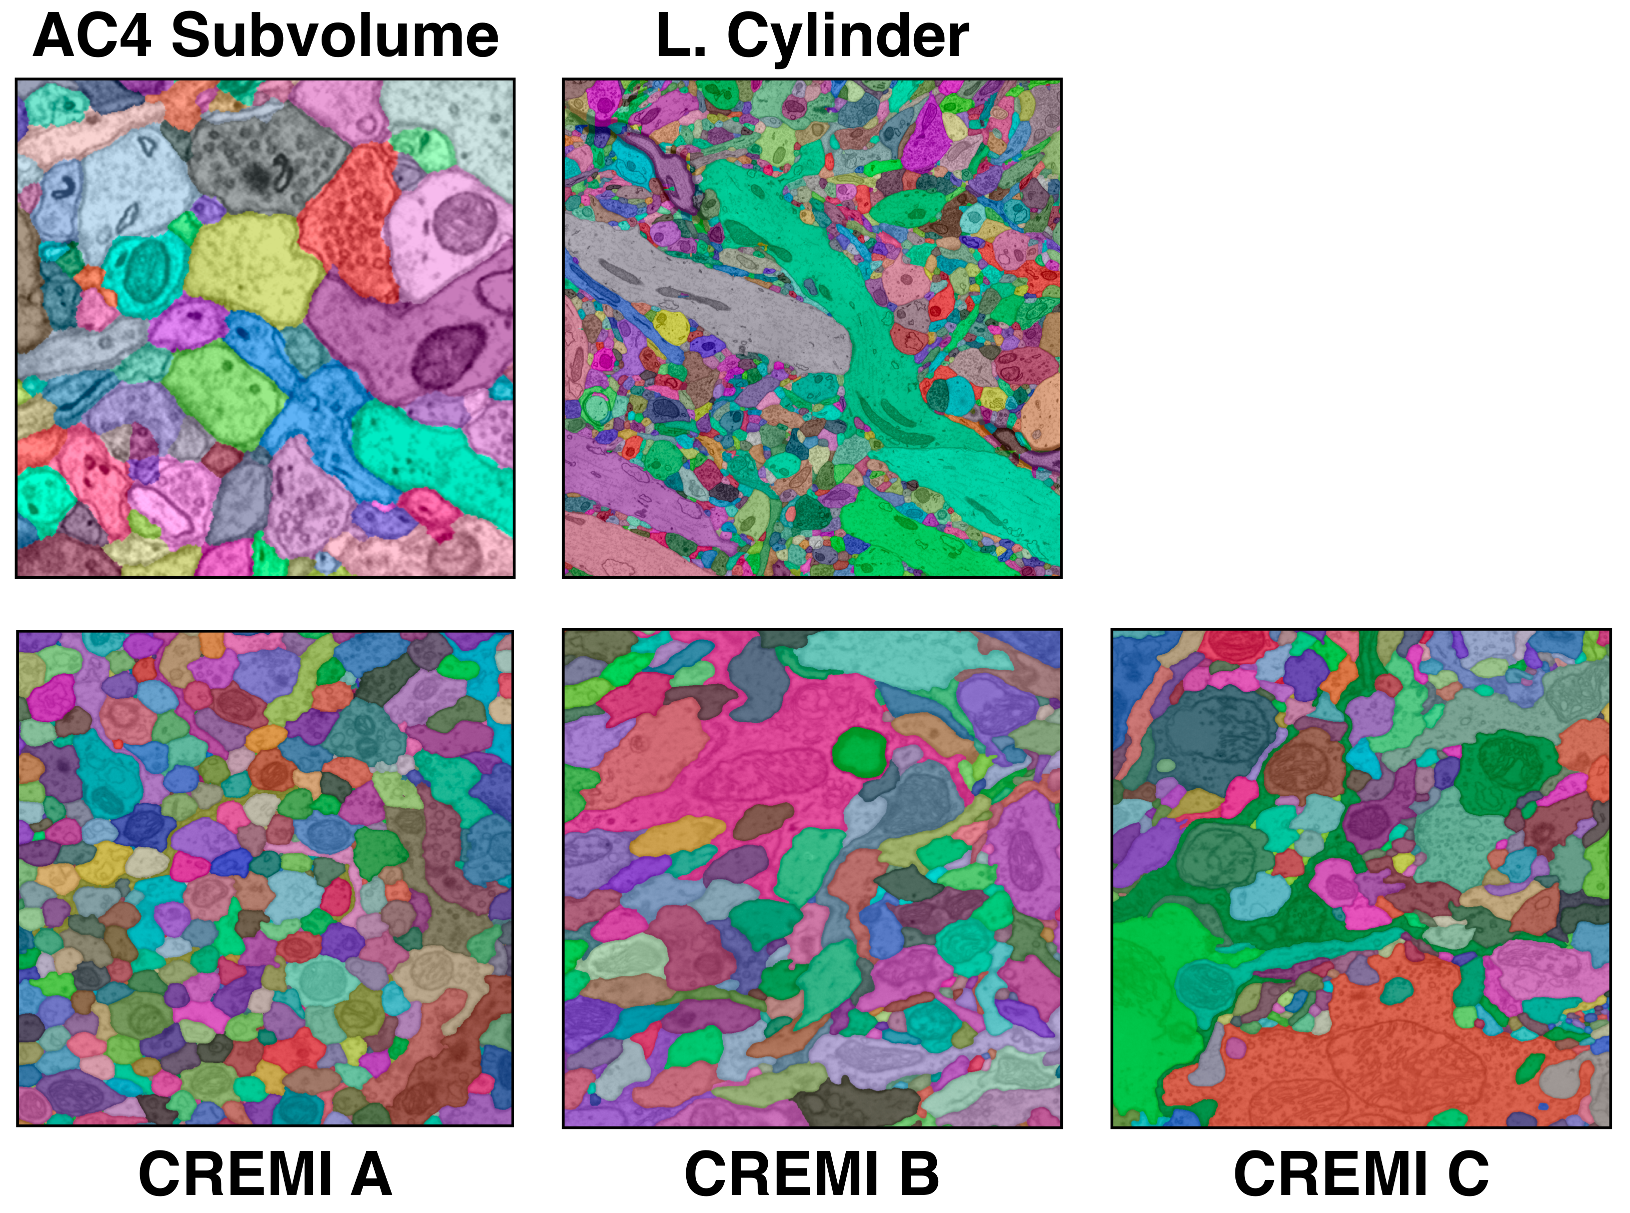
\includegraphics[width=\linewidth]{gfx/datasets.png}
\caption{The five different datasets we use for evaluation. The top row shows the first slice of the AC4 and L.~Cylinder mouse brain datasets as reported in the paper. The bottom row shows the first slice of the CREMI A/B/C fruit fly datasets which we used for additional experiments.}
\label{fig:datasets}
\end{figure}

We report experiments and results on the L.~Cylinder dataset in the paper. Figure~\ref{fig:cyltrails} and~\ref{fig:cylboxplot} visualize the reported results measured as variation of information (VI). We compare automatic selection with threshold and selection oracle using focused proofreading and guided proofreading.

\paragraph{Best possible VI.} The selection oracle using guided proofreading does not reach the best possible VI score. We calculate this score by intersecting the initial segmentation and the ground truth. In theory, the classifier should be able to reach this lower bound. However, due to the classification patch size, the membrane probability maps we used included a 30 pixel frame region. Guided proofreading ignores all segments within this frame region, and so cannot reach the best possible VI in some datasets.

\begin{figure}[t]
\centering
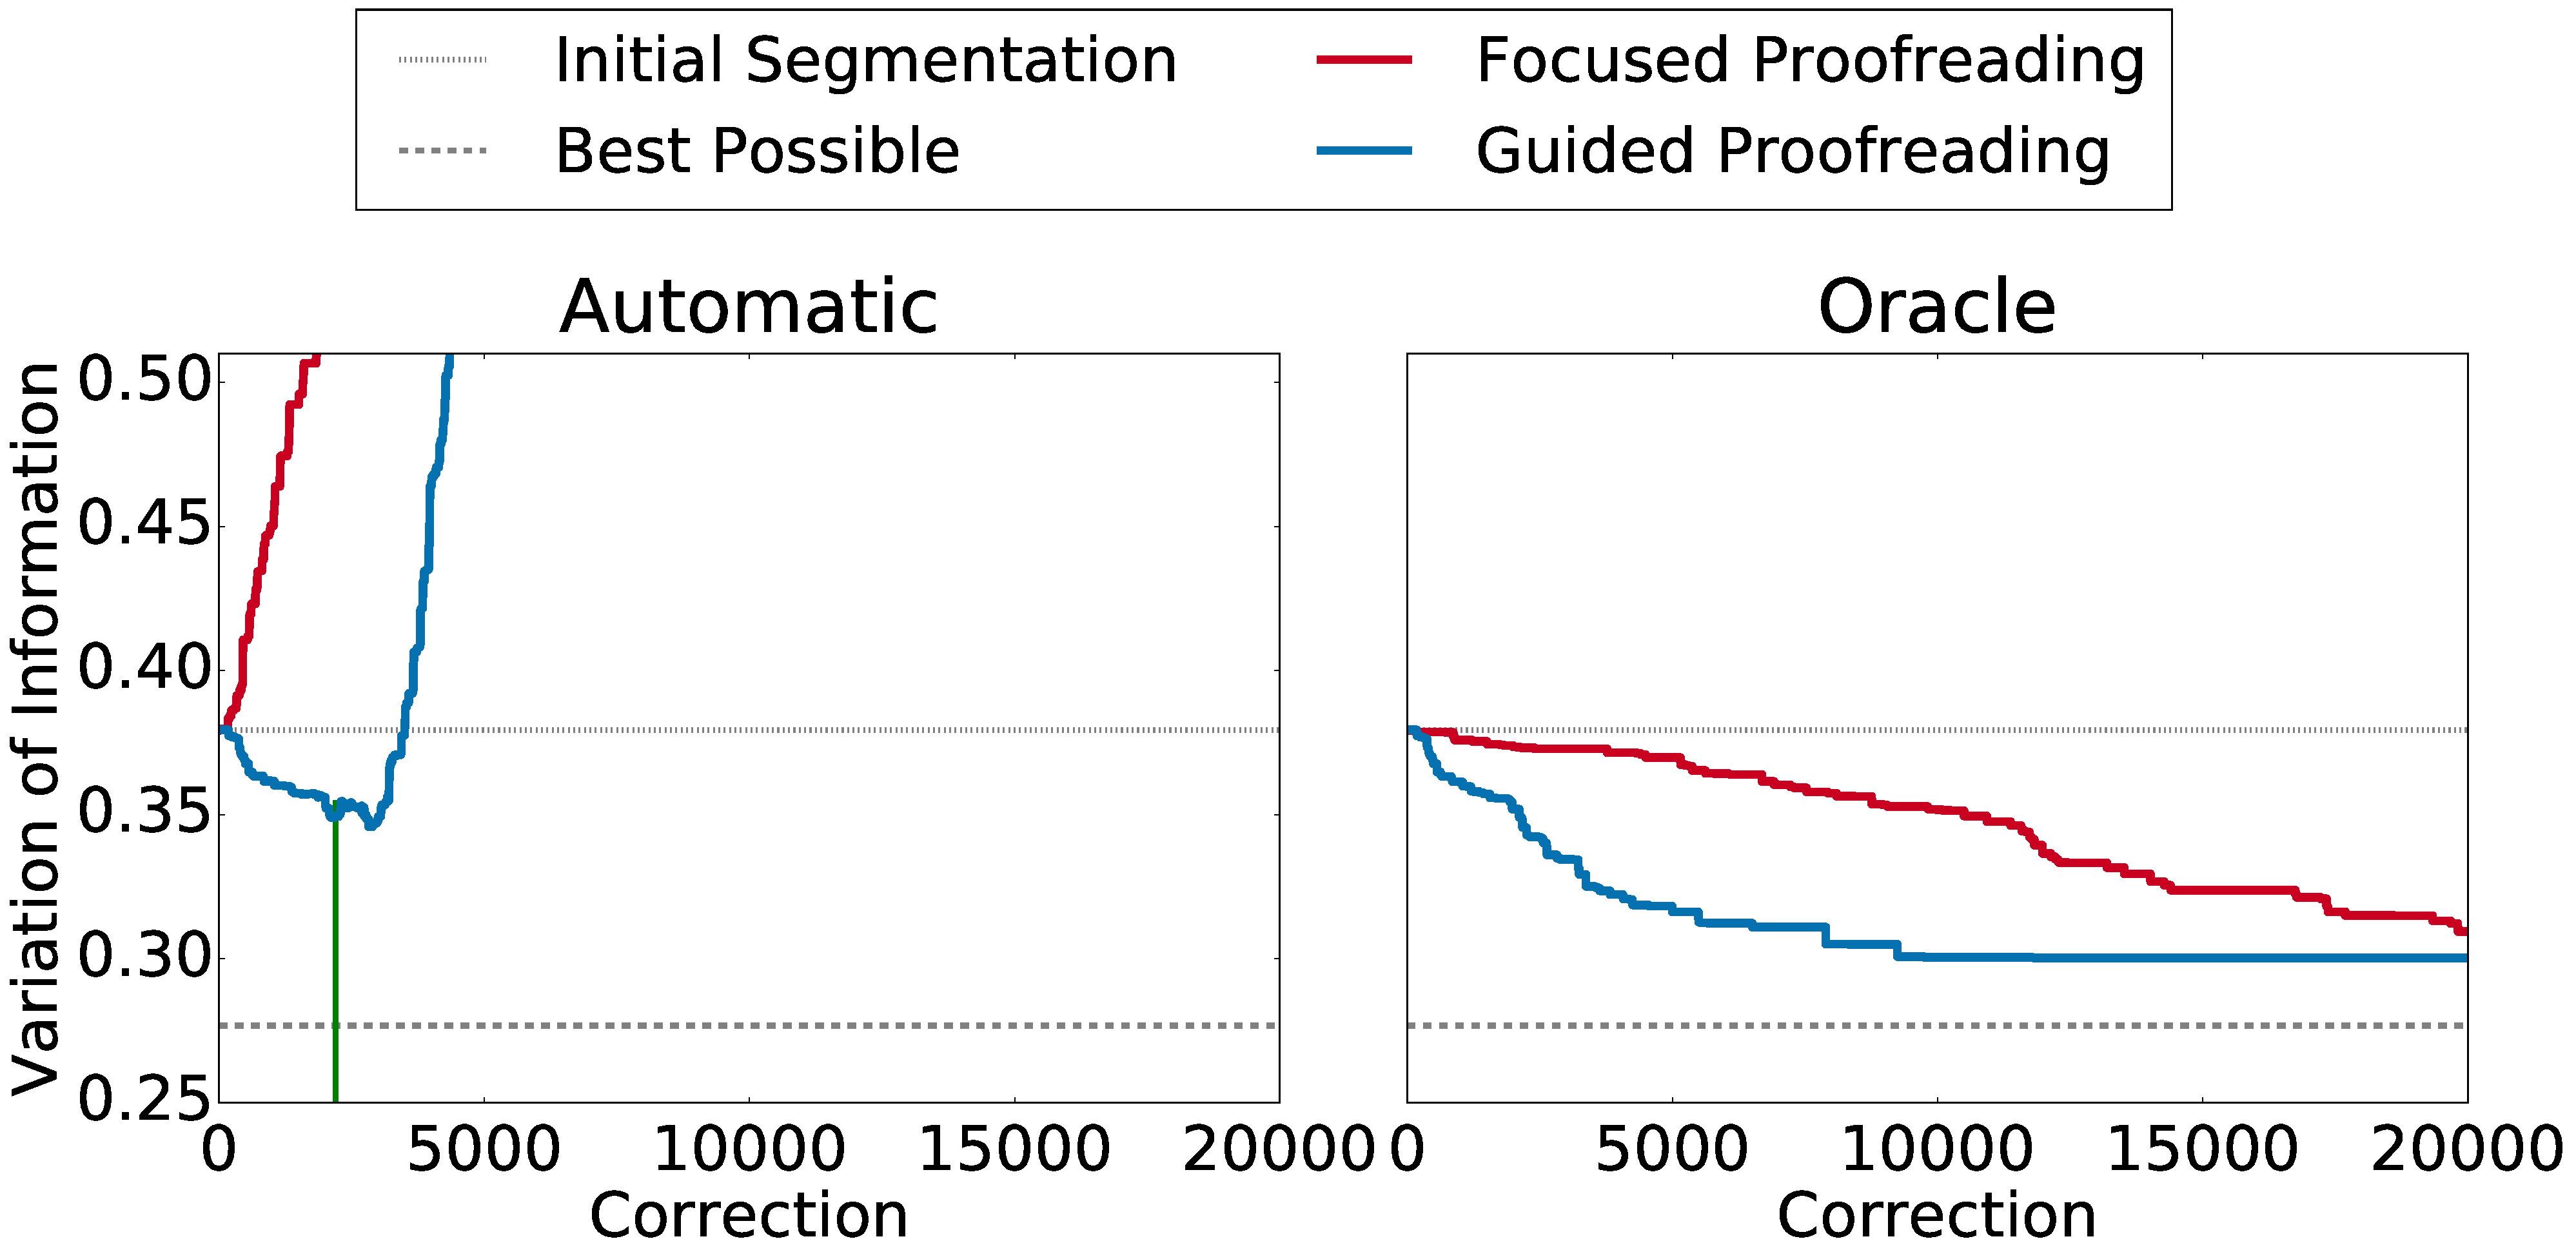
\includegraphics[width=\linewidth]{gfx/cyl_trails.pdf}
\caption{Performance comparison of Plaza's focused proofreading and our guided proofreading on the L.~Cylinder dataset as reported in the paper. All measurements are shown as median VI, the lower the better. We compare automatic selection with threshold ($p_t=0.95$, green line) and the selection oracle for accepting or rejecting corrections using each method. Guided proofreading yields better results faster with fewer corrections.}
\label{fig:cyltrails}
\end{figure}

\begin{figure}[t]
\centering
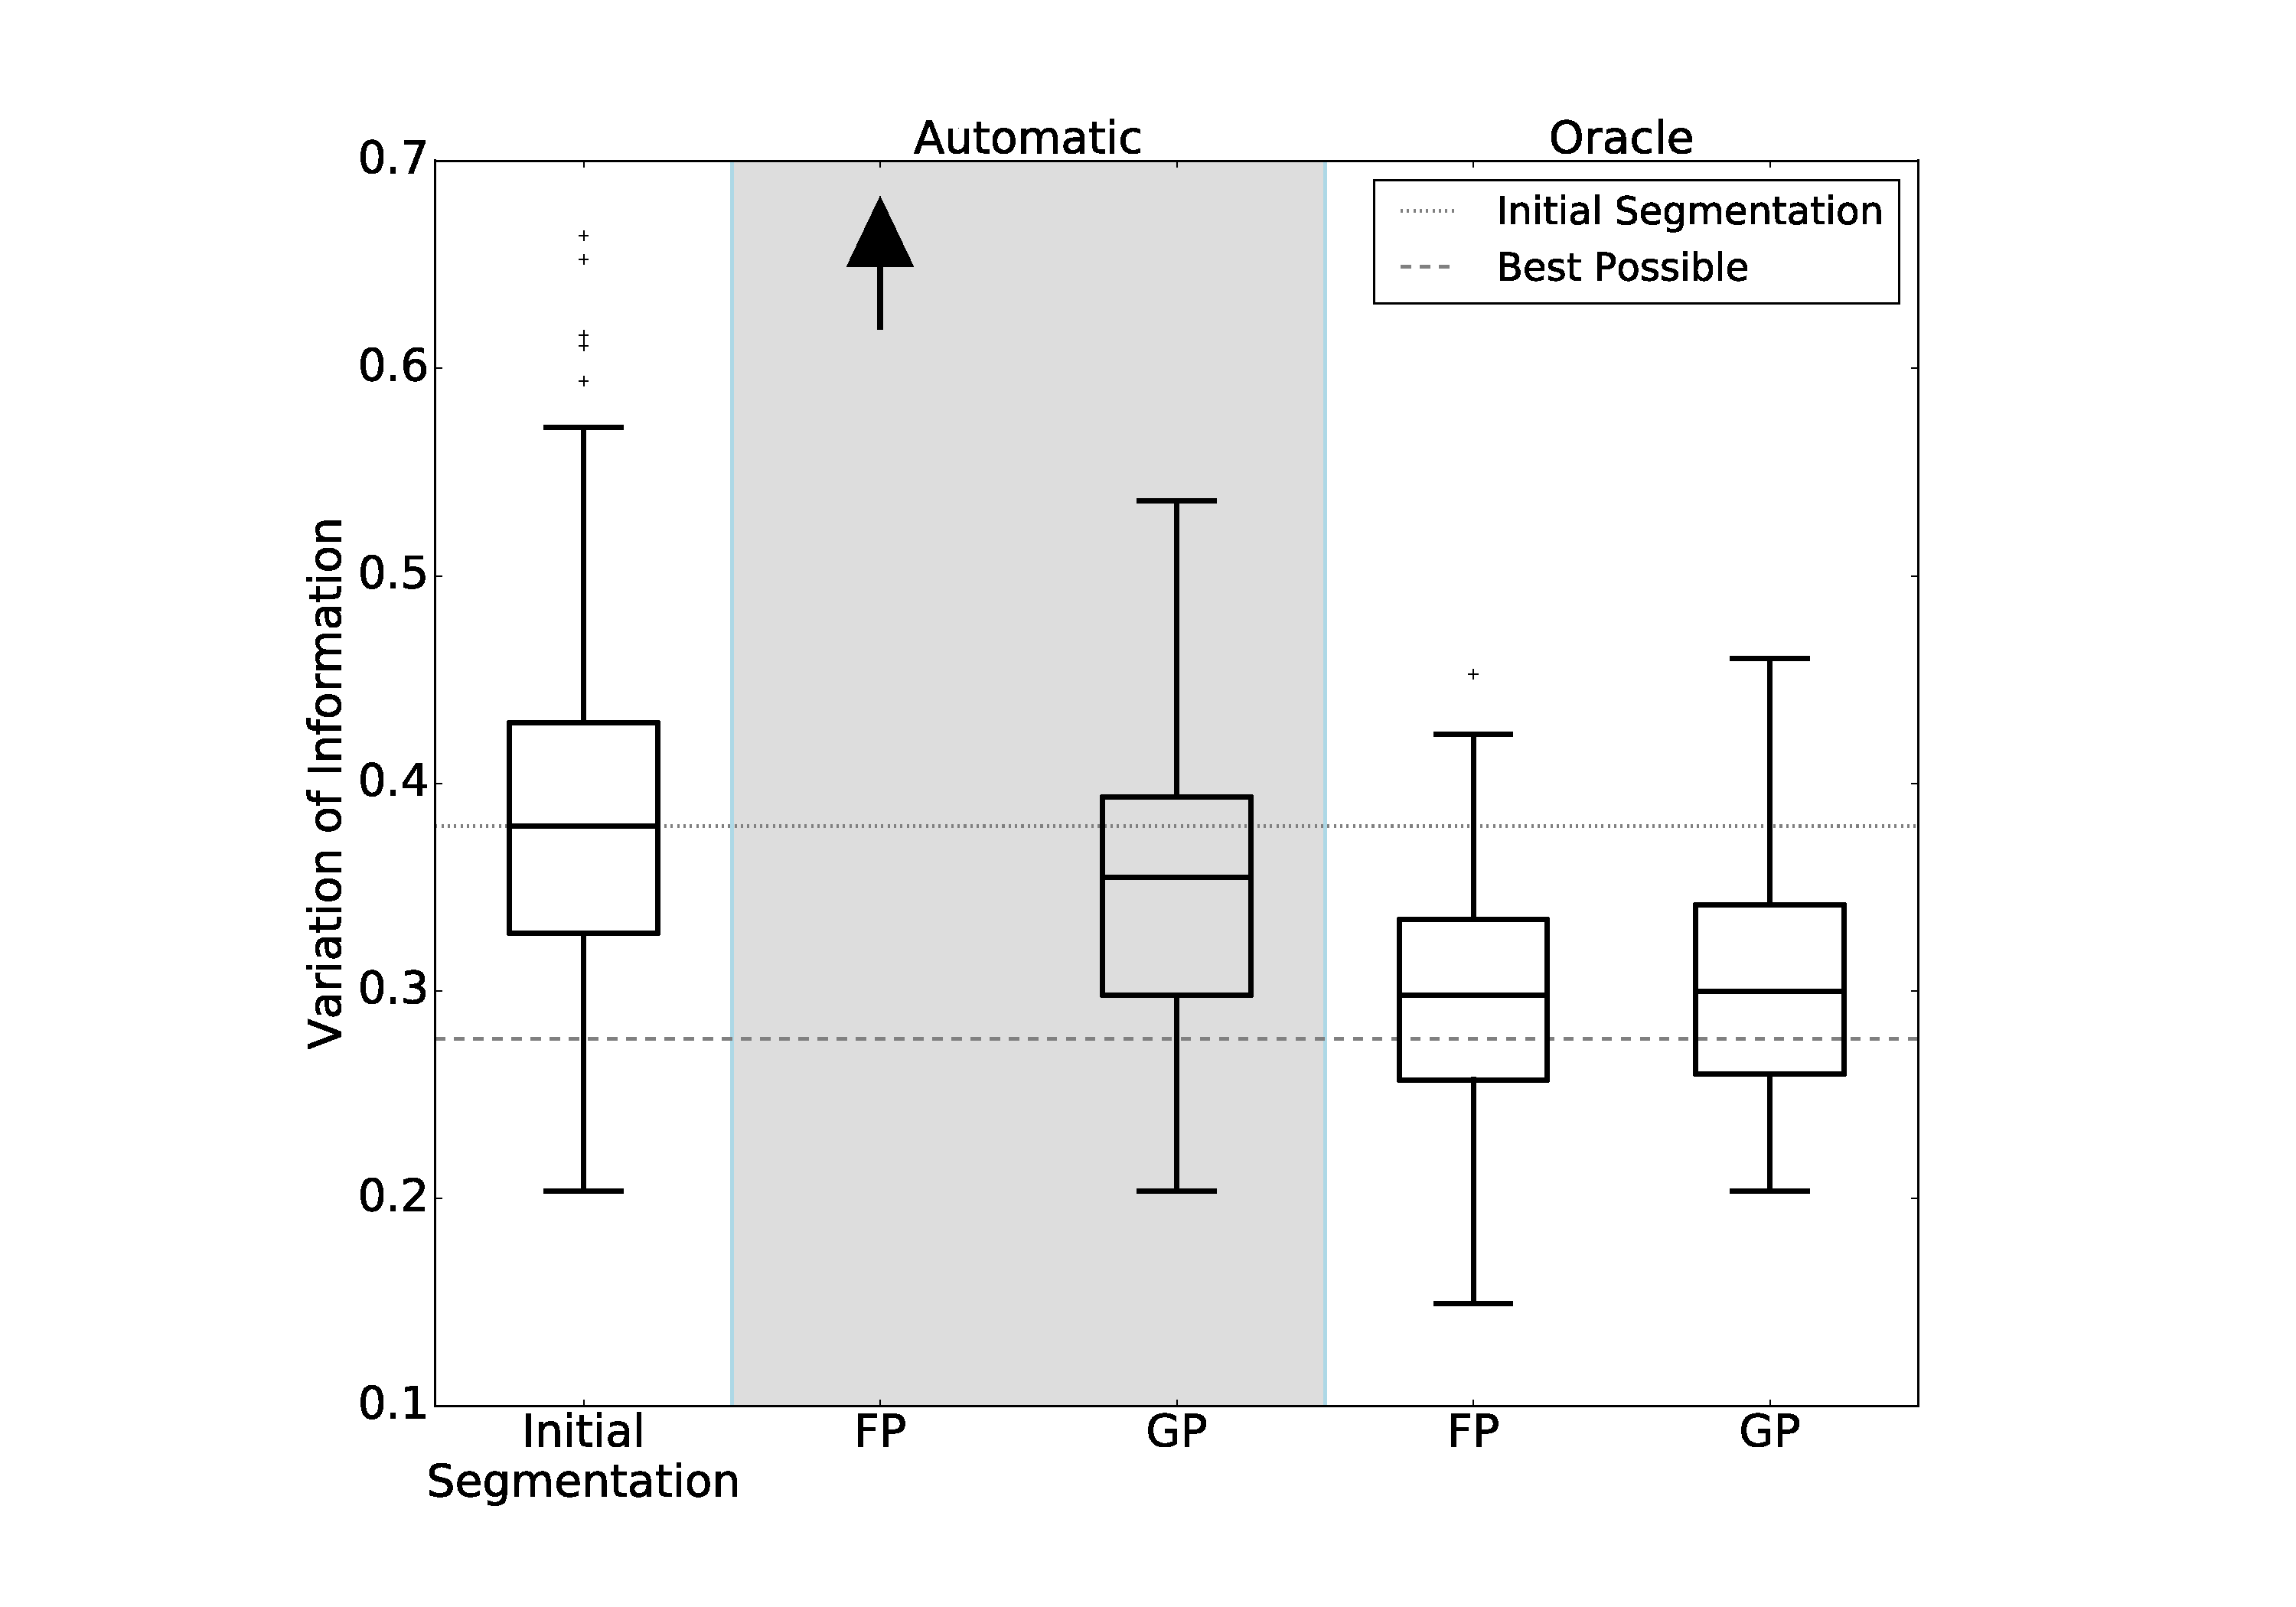
\includegraphics[width=\linewidth]{gfx/cylboxplot.pdf}
\caption{VI distributions of guided proofreading (GP) and focused proofreading (FP) output across slices of the L.~Cylinder dataset, with different error correction approaches. The variation resulting from performance of FP with automatic selection is $7.8\times$ higher than GP (\protect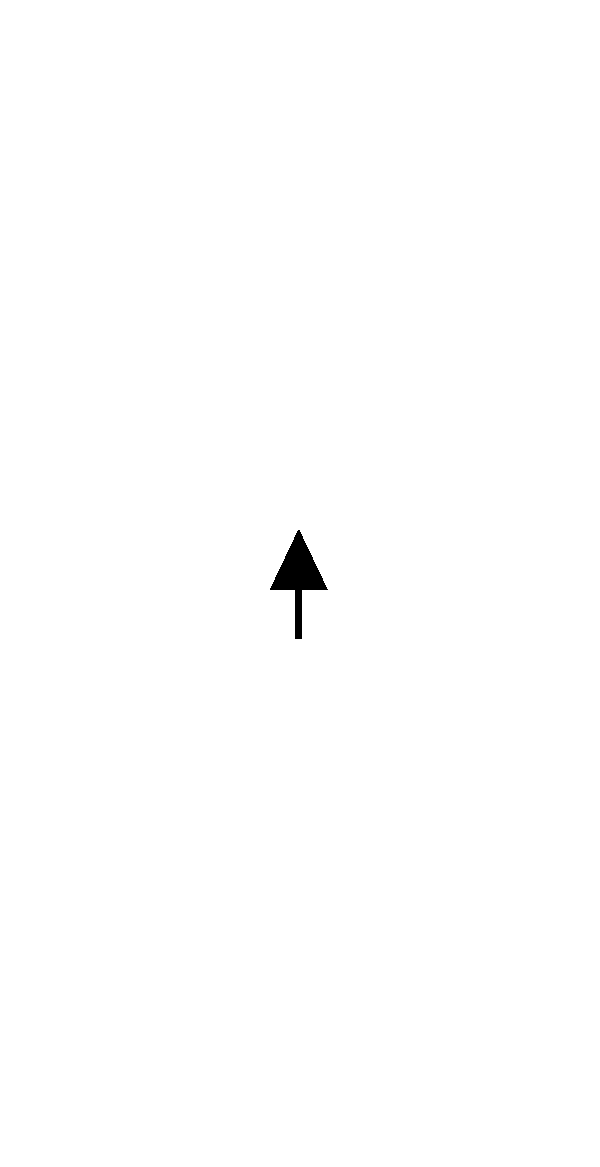
\includegraphics[width=0.2cm]{gfx/arrow.pdf}), with median VI of $2.75$ and $SD=0.789$.}
\label{fig:cylboxplot}
\end{figure}

\section{Confirmatory Data Analysis} 

We use a single factor between-subject design with the factor being the proofreading method (GP, FP, or Dojo). Our hypothesis is that VI reduction is significantly better with GP than with other tools. For this, we treat VI as a continuous variable and use analysis of variance (ANOVA~\cite{shaffer1995}) followed by parametric tests (Welch's t-test~\cite{welch}).

\paragraph{AC4 subvolume.} For novice performance, we observe a significant effect ($\alpha=0.05$) of which proofreading tool is used for the three conditions GP, FP, and Dojo [$F(2,27) = 6.446, p = 0.005$] when comparing the mean VI outcome. Post hoc comparisons (after Bonferroni correction) indicate that the mean VI for GP is significantly lower than for FP [$t_{27} = -2.7696, p = 0.0168$], and that the mean VI for GP is significantly lower than for Dojo [$t_{27} = -4.407, p < 0.001$]. This means that novices using GP perform significantly better than using FP and Dojo.
A similar trend is visible when comparing the expert performance between GP and FP as the change in mean VI of GP is significantly better ([$F(1,18) = 7.054, p = 0.016$] and [$t_{18} = -2.6559, p = 0.0216$]). For automatic selection with threshold, the difference in mean VI is very large and GP also performs significantly better ([$F(1,18) = 89.902, p < 0.001$] and [$t_{18} = 9.482, p < 0.001$]). The final VI scores of the selection oracle with GP and FP are very similar and the difference between them is not significant [$F(1,18) = 0.795, p = 0.384$]. However, the VI reduction rate of GP is much higher (Fig.~6, main paper, right).

\vspace{-4mm}

\paragraph{L. Cylinder.} The automatic selection with threshold yields similar results as on the AC4 dataset, and we observe a significant improvement when using GP instead of FP ([$F(1,98) = 26.676, p < 0.001$], post hoc comparison [$t_{98} = 5.1648, p < 0.001$]). The selection oracles of GP and FP result in very similar final VI scores and the difference is not significant [$F(1,98) = 0.071, p = 0.790$], but GP reaches minimum VI faster in $10,000$ corrections versus FP in $26,170$ corrections.
    
    